\section{Stati, Autostati, Osservabili e Indeterminazione}
È arrivato il momento di introdurre la \textbf{notazione di Dirac} \index{notazione di Dirac}.

Siccome si tratta solo di un formalismo non è data una definizione matematica. Semplicemente, approfittando del fatto che gli stati formano uno spazio vettoriale si stabilisce un modo per indicare i "vettori" di questo spazio, che saranno gli stati:
\[
	|\psi \ket
\]
Questo oggetto è chiamato un "ket", e risponde alla definizione classica di vettore. Viene introdotta anche la notazione per i vettori duali, o covettori, chiamati "bra":
\[
	\bra \psi |
\]
Sulla base delle affermazioni fatte in precedenza si può dire che è possibile definire un prodotto interno:
\[
	|\psi\ket \cdot |\xi\ket = \braket \psi \xi = \rnint \xi \psi^*
\],
Inoltre siccome lo spazio è unitario è sempre possibile generare una base, allora si indica con $|\psi_j\ket$ il vettore generico della base, con $j \in J$ insieme generico, non necessariamente numerabile.
(si ricorda che gli stati sono funzioni $\L^p$) e anche un prodotto esterno:
\[
	\Ket \psi \times \Ket \xi = \ketbra \psi \xi
\]
tale che per ogni stato $\Ket \chi$
\[
	\ketbra \psi \xi \Ket \chi = \braket \xi \chi \Ket \psi
\]
Se nella definizione di prodotto esterno di usano al posto di $\Ket \psi$ e $\Ket \xi$ gli elementi della base $\Ket {\psi_j}$ risulta che è possibile definire le proiezioni canoniche sulla base di un dato stato, ottenendo i "proiettori".\index{notazione di Dirac ! Proiettori}
\[
	\Ket \xi = 
	\begin{pmatrix}
		\ketbra{\psi_1}{\psi_1}\ \Ket{\xi} \\
		\ketbra{\psi_2}{\psi_2}\ \Ket{\xi} \\
		\ketbra{\psi_3}{\psi_3}\ \Ket{\xi} \\
		\vdots
	\end{pmatrix}
	= 
	\begin{pmatrix}
		\crossToScalket{\psi_1}{\psi_1}{\xi} \\
		\crossToScalket{\psi_2}{\psi_2}{\xi} \\
		\crossToScalket{\psi_3}{\psi_3}{\xi} \\
		\vdots
	\end{pmatrix}
\]
Un operatore lineare può essere scritto come:
\[
	\hat A = \sum_{i,j \in J} a_{ij} \ketbra{\psi_i}{\psi_j}
\]
dove gli $a_{ij}$ sono coefficienti caratteristici dell'operatore.\\
Se la base utilizzata è la base degli autovettori di $A$ risulta comodamente:
\[
	\hat A = \sum_{j \in J} a_{j} \ketbra{\psi_j}{\psi_j}
\]
dove gli $a_{j}$ sono gli autovalori associati agli autostati $\Ket \psi_j$.
\tab
L'ultimo risultato interessante è il fatto che se lo spazio degli stati è a dimensione finita, allora questi assumono la forma di veri e propri vettori (vettori colonna per i ket e vettori riga per i bra), le cui componenti sono esprimibili, una volta definita una base, grazie ai proiettori; di conseguenza gli operatori lineari vengono rappresentati da matrici. Passare da un bra a un ket e viceversa coincide col calcolare il trasposto coniugato del vettore (indicato con $^\dag$).
\tab

È essenziale notare e tenere sempre conto del fatto che il vettore $\Ket \psi$ non è formalmente legato alla funzione d'onda $\psi(x,t)$: ciò che viene trascritto tra i bra e i ket sono dei "tag", dei nomi, finalizzati a identificare il vettore e a distinguerlo dagli altri, niente di più.



\subsection*{Spin degli Elettroni} \index{spin degli Elettroni}
Nel 1922 gli scienziati Otto Stern e Walther Gerlach hanno ideato un esperimento finalizzato a trovare quale fosse il momento magnetico dell'elettrone. Hanno costruito un apparato che avrebbe deviato un flusso di elettroni in funzione del loro momento magnetico lungo l'asse $z$. Il risultato atteso era che ogni elettrone avrebbe avuto un momento magnetico divero, seguento una distribuzione casuale, possibilmente gaussiana.\\
Invece il risultato ottenuto fu che il fascio di elettroni di divideva in due fasci soltanto con equa distribuzione, quindi che ogni elettrone aveva uno di due valori di momento magnetico.

\begin{figure}[h]
	\centering
	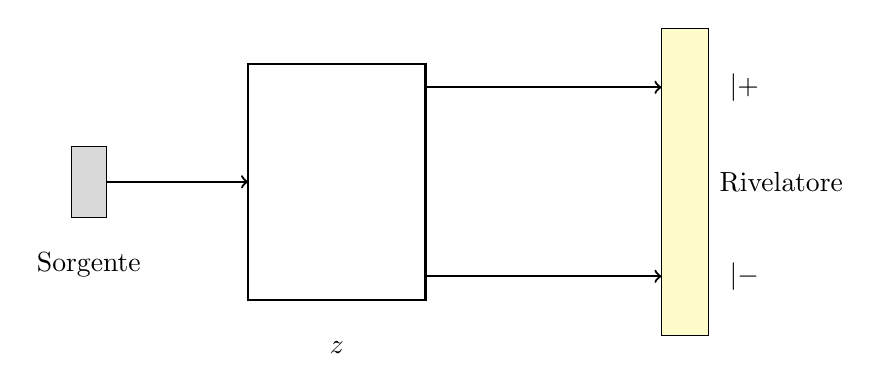
\begin{tikzpicture}[scale=1.5]
		% Electron source
		\draw[fill=gray!30] (-3,-0.3) rectangle (-2.7,0.3);
		\node at (-2.85,-0.7) {Sorgente};
		
		% Incoming electrons
		\draw[->,thick] (-2.7,0) -- (-1.5,0);
		
		% Magnetic field region
		\draw[thick] (-1.5,-1) rectangle (0,1);
		\node at (-0.75,-1.4) {$\SG z$};
		
		% Upper beam (spin up)
		\draw[->,thick] (0,0.8) -- (2,0.8);
		\node at (2.7,0.8) {$|+\ket$};
		
		% Lower beam (spin down)
		\draw[->,thick] (0,-0.8) -- (2,-0.8);
		\node at (2.7,-0.8) {$|-\ket$};
		
		% Detector
		\draw[fill=yellow!20] (2,-1.3) rectangle (2.4,1.3);
		\node at (2.7,0) {\ \ \ \ \ \ \ \ Rivelatore};
	\end{tikzpicture}
	\caption{Schema dell'apparato di Stern-Gerlach. Il flusso di elettroni viene deviato dal campo magnetico secondo lo spin.}
\end{figure}

In particolare, misurando il momento magnetico associato alla deviazione, risulta che gli elettroni possono avere momento magnetico di $\pm$ \thhalf. Che cosa succede se proviamo a generare uno spazio degli stati a partire da questi risultati?
Una possibile base per questo spazio è:
\[
	|+\ket = \begin{pmatrix} 1 \\ 0 \end{pmatrix}, \ \ \ \ |-\ket = \begin{pmatrix} 0 \\ 1 \end{pmatrix}
\]
Al chè si ha la rappresentazione, per esempio, dell'operatore di Stern e Gerlach $\SG z$:
\[
	\hat S_z = \frac{\hslash}{2} |+\ket \bra +| - \frac{\hslash}{2} |-\ket \bra -| = \frac{\hslash}{2} \begin{pmatrix} 1 & 0 \\ 0 & -1 \end{pmatrix} = \frac{\hslash}{2} \sigma_z
\]

\subsection*{Misurazione degli Osservabili}
Dato uno stato generico $|\vphi \ket$ e un operatore osservabile $\hat A$ con autostati $|\psi_j \ket$ (si nota che un ossservabile per essere tale deve essere un operatore hermitiano, cosicchè gli autovalori risultino reali e gli autostati ortogonali) e autovalori $a_j$, quel che accade durante una misurazione è che lo stato $|\vphi \ket$ collassa in uno degli autostati $|\psi_j \ket$ con probabilità $p_j = |\bra \psi_j | \vphi \ket|^2$. Nel caso di un apparato di misura discreto, il risultato della misura è il valore dell'autovettore associato all'autostato in cui $\vphi$ è collassato.

Riassumendo, gli assiomi della misurazione, posto lo stato del sistema rappresentato da un Ket in uno spazio di Hilbert, e un operatore hermitiano:
\begin{enumerate}
	\item La misurazione di un osservabile consiste nel "leggere" uno degli autovalori possibili dell'osservabile;
	\item A seguito della misurazione, lo stato è permanentemente e irrevocabilmente modificato, e diventa l'autostato associato all'autovalore misurato;
	\item La probabilità di misurare un autovalore piuttosto che un altro è il modulo quadro della proiezione dello stato sull'autostao associato.
\end{enumerate}

\subsubsection*{Esempio: esperimento di Stern e Gerlach}
Si considerino lo stato $|\psi\ket$ e l'opereatore $\hat S_z$ descritto sopra. Risulta:
\begin{equation*}
	\hat S_z |\psi\ket = \frac{\hslash}{2} |+_z\ket \bra +_z| \psi\ket - \frac{\hslash}{2} |-_z\ket \bra -_z| \psi\ket
\end{equation*}
Quindi si può usare d'ora in poi la base $B_z = \{|+_z\ket, |-_z\ket\}$.\\
Ora si prenda l'operatore $\hat S_x$. Questo ha una nuova base di autostati $B_x$, in cui si rappresenta come:
\[
	\hat S_x = \frac{\hslash}{2} |+_x\ket \bra +_x| - \frac{\hslash}{2} |-_x\ket \bra -_x|
\]
E bisogna valutare il significato di $|+_x\ket$ e $|-_x\ket$ nella base $B_z$.\\
Dall'esperimento di Stern e Gerlach fatto applicando prima $\hat S_z$ e poi $\hat S_x$ si sa che se si misura $S_x$ su uno stato $|+_z\ket$ si ottiene con probabilità 1/2 sia $|+_x\ket$ che $|-_x\ket$. Quindi si può scrivere:
\begin{align*}
	|+_x\ket = \frac{1}{\sqrt 2} (|+_z\ket + e^{i\theta}|-_z\ket) \\
	|-_x\ket = \sqrthalf (|+_z\ket + e^{i\tau}|-_z\ket)
\end{align*}
con
\[
	0 = \bra +_x | -_x \ket = \half (\bra+_z| + e^{-i\theta}\bra-_z|)(|+_z\ket + e^{i\tau}|-_z\ket) = \]\[
	= \half (\bra+_z| |+_z\ket + e^{i\tau}\bra+_z| |-_z\ket + e^{-i\theta}\bra-_z| |+_z\ket -_z e^{-i\theta}e^{i\tau}\bra-_z| |-_z\ket) = 1 + e^{i(\tau - \theta)} \]\[
	\implies e^{i(\theta - \tau)} = -1 \implies \theta - \tau = \pi
\]
e quindi
\begin{align*}
	\hat S_x = \frac{\hslash}{2} \begin{pmatrix} 0 & e^{i(\theta - \tau)} \\ e^{-i(\theta - \tau)} & 0 \end{pmatrix}
\end{align*}
Risulta comodo in questo caso porre $\theta = \pi$ e $\tau = 0$ e quindi
\[
	\hat S_x = \frac{\hslash}{2} \begin{pmatrix} 0 & 1 \\ 1 & 0 \end{pmatrix} = \frac{\hslash}{2} \sigma_y
\]

Per quanto riguarda invece $\hat S_y$ si può procedere in modo analogo; ponendo la perpendicolarità con $\hat S_x$ si ottiene $\theta = \pi/2$ e $\tau = -\pi/2$, quindi
\[
	\hat S_y = \frac{\hslash}{2} \begin{pmatrix} 0 & -i \\ i & 0 \end{pmatrix} = \frac{\hslash}{2} \sigma_x
\]
E, per completezza si aggiunge $\hat S_z$:
\[
	\hat S_z = \frac{\hslash}{2} \begin{pmatrix} 1 & 0 \\ 0 & -1 \end{pmatrix} = \frac{\hslash}{2} \sigma_z
\]

\subsubsection*{Osservabili compatibili}
Dati due osservabili hermitiani che commutano ($[\hat A, \hat B] = 0$), esiste una base di autostati comune, in cui se uno è diagonale allora anche l'altro e diagonale.
\begin{proof}
	Mostrare che se $\Ket {a_{j}}$ è autostato di $\hat A$ allora lo è anche di $\hat B$.
\end{proof}

\subsubsection*{Interferenza degli osservabili}
Questa procedura dimostra il fatto fisico per cui l'introduzione di un osservabile può interferire con le misurazioni.

Sia allora un sistema con tre osservabili: $\hat A, \hat B, \hat C$. Siano $\Ket {a_{\scriptscriptstyle n}}$, $\Ket {b_{\scriptscriptstyle n}}$ e $\Ket {c_{\scriptscriptstyle n}}$ le rispettive basi diagonalizzanti. Allora nella prima configurazione si applicano $\hat A, \hat B$ e poi $\hat C$ a un sistema nello stato $\Ket {\psi_0} = \Ket {a_{\scriptscriptstyle 0}}$; risulta che la probabilità di misurare $\Ket{c_{\scriptscriptstyle 0}}$ è data da:
\[
	\P(\Ket {c_{\scriptscriptstyle 0}}) = \sum_{n}\abs{\braket{c_{\scriptscriptstyle 0}}{b_{\scriptscriptstyle n}}\braket{b_{\scriptscriptstyle n}}{a_{\scriptscriptstyle 0}}}^2
\]
in quanto nel passaggio da $\hat B$ potrebbe aver assunto qualsiasi stato intermedio, senza distinzione.

Nella seconda configurazione invece di applicano solo $\hat A$ e $\hat C$, cosicchè la probailità stavolta è data da solo $\P(\Ket {c_{\scriptscriptstyle 0}}) = \abs{\braket{c_{\scriptscriptstyle 0}}{a_{\scriptscriptstyle 0}}}^2$. Ora è possibile inserire due completezze in questa maniera:
\[
	\abs{\braket{c_{\scriptscriptstyle 0}}{a_{\scriptscriptstyle 0}}}^2 = \braket{c_{\scriptscriptstyle 0}}{a_{\scriptscriptstyle 0}}\braket{a_{\scriptscriptstyle 0}}{c_{\scriptscriptstyle 0}} = \sum_{n,m}\braket{c_{\scriptscriptstyle 0}}{b_{\scriptscriptstyle n}}\braket{b_{\scriptscriptstyle n}}{a_{\scriptscriptstyle 0}}\braket{a_{\scriptscriptstyle 0}}{b_{\scriptscriptstyle m}}\braket{b_{\scriptscriptstyle m}}{c_{\scriptscriptstyle 0}}
\]
E separando la doppia sommatoria nei casi $n=m$ e $n\neq m$ risulta:
\[
	\P(\Ket {c_{\scriptscriptstyle 0}}) = \sum_{n}\abs{\braket{c_{\scriptscriptstyle 0}}{b_{\scriptscriptstyle n}}\braket{b_{\scriptscriptstyle n}}{a_{\scriptscriptstyle 0}}}^2 + \sum_{n\neq m}\braket{c_{\scriptscriptstyle 0}}{b_{\scriptscriptstyle n}}\braket{b_{\scriptscriptstyle n}}{a_{\scriptscriptstyle 0}}\braket{a_{\scriptscriptstyle 0}}{b_{\scriptscriptstyle m}}\braket{b_{\scriptscriptstyle m}}{c_{\scriptscriptstyle 0}}
\]
È evidente che la prima sommatoria è identica a quella della prima configurazione! In sostanza la rimozione dell'operatore $\hat B$ ha introdotto una serie di termini d'interferenza, uno dei molto apparenti paradossi della meccanica quantistica.\\
È opportuno notare il fatto che se $\hat B$ commuta con $\hat A$ (oppure con $\hat C$) la seconda sommatoria si annulla, in quanto $\Ket {a_{\scriptscriptstyle n}}$ sarebbe anche base diagonalizzante per $\hat B$, quindi per $m \neq n$ si avrebbe che almeno uno tra i due termini $\braket{b_{\scriptscriptstyle n}}{a_{\scriptscriptstyle 0}}$ e $\braket{a_{\scriptscriptstyle 0}}{b_{\scriptscriptstyle m}}$ deve essere 0, perché i $\Ket {b_{\scriptscriptstyle n}}$ non sarebbero altro che una permutazione degli $\Ket {a_{\scriptscriptstyle n}}$, ovvero, solo gli osservabili non compabili modificano lo stato del sistema!